\chapter{Risk factors: fruits}
\label{applications-log_normal}

Although the primary focus of the meta-regression framework developed
in this book is for estimating prevalence of disease, it is also
useful for estimating other age-specific quantities of interest in
descriptive epidemiology.  Subsequent chapters will address the
consistent estimation framework which allows data on incidence,
remission, and mortality to be included in estimates of prevalence;
this approach produces estimates of age-specific incidence, remission,
and mortality as ancillary outputs.  But before turning to that,
this chapter considers the possibility of using the
age-standardizing mixed effects spline model to produce estimates of
risk factor exposures.

An important component of the GBD 2010 Study was the estimation of
disease burden attributable to risk factors, such as the lack of fresh
fruit.  Fruit consumption is a non-negative quantity, so it is
acceptable to model it with the negative binomial rate model.  This is
somewhat inelegant, however, because this model assumes that the
underlying quantity being measured is count data.  A count model is
appropriate for prevalence and incidence rates, which represent, for
example, how many cases were observed during a certain period of
observation.  However, a continuous distribution, such as one of the
transformed normal models from Chapter~\ref{theory-rate_model}, is
more common for modeling a quantity like kilograms of fruit consumed
per day per capita.  In this chapter, we will compare the results of
using the negative binomial rate model with two more traditional
models for continuous data, the normal model and the log-normal model.

Fruit consumption has a significant protective
effect against morbidity and mortality from several diseases.
Measured as the total intake of fruit per day (kg/day), fruit
includes all fresh, frozen, cooked, canned or dried fruits, excluding
fruit juices and salted or pickled fruits. \cite{he_increased_2007,
  boeing_intake_2006}

Systematic review for
risk factor epidemiology proceeds much the same as for disease
prevalence, at least for determining the population level exposure to
the risk.  In the case of lack of fruit, systematic review collected
$1502$ data points on age-specific consumption of fruit.

Often it is useful to design statistical models based on real world
processes, using count models for discrete data and rate models for
continuous data as discussed in Chapter~\ref{theory-rate_model}.
Since fruit consumption is a continuous variable, one may choose the
log normal or normal rate model over the negative binomial model to
maintain a mechanistic understanding of the statistical model.  The
models differ in their treatment of numbers that are very close to
zero, but, with well-behaved data, the model estimates are largely
independent of the choice of rate model, as seen in
Figure~\ref{fig:app-fruit rate type}, which compares estimates for
models fit to data from the United States.

    \begin{figure}[h]
        \begin{center}
            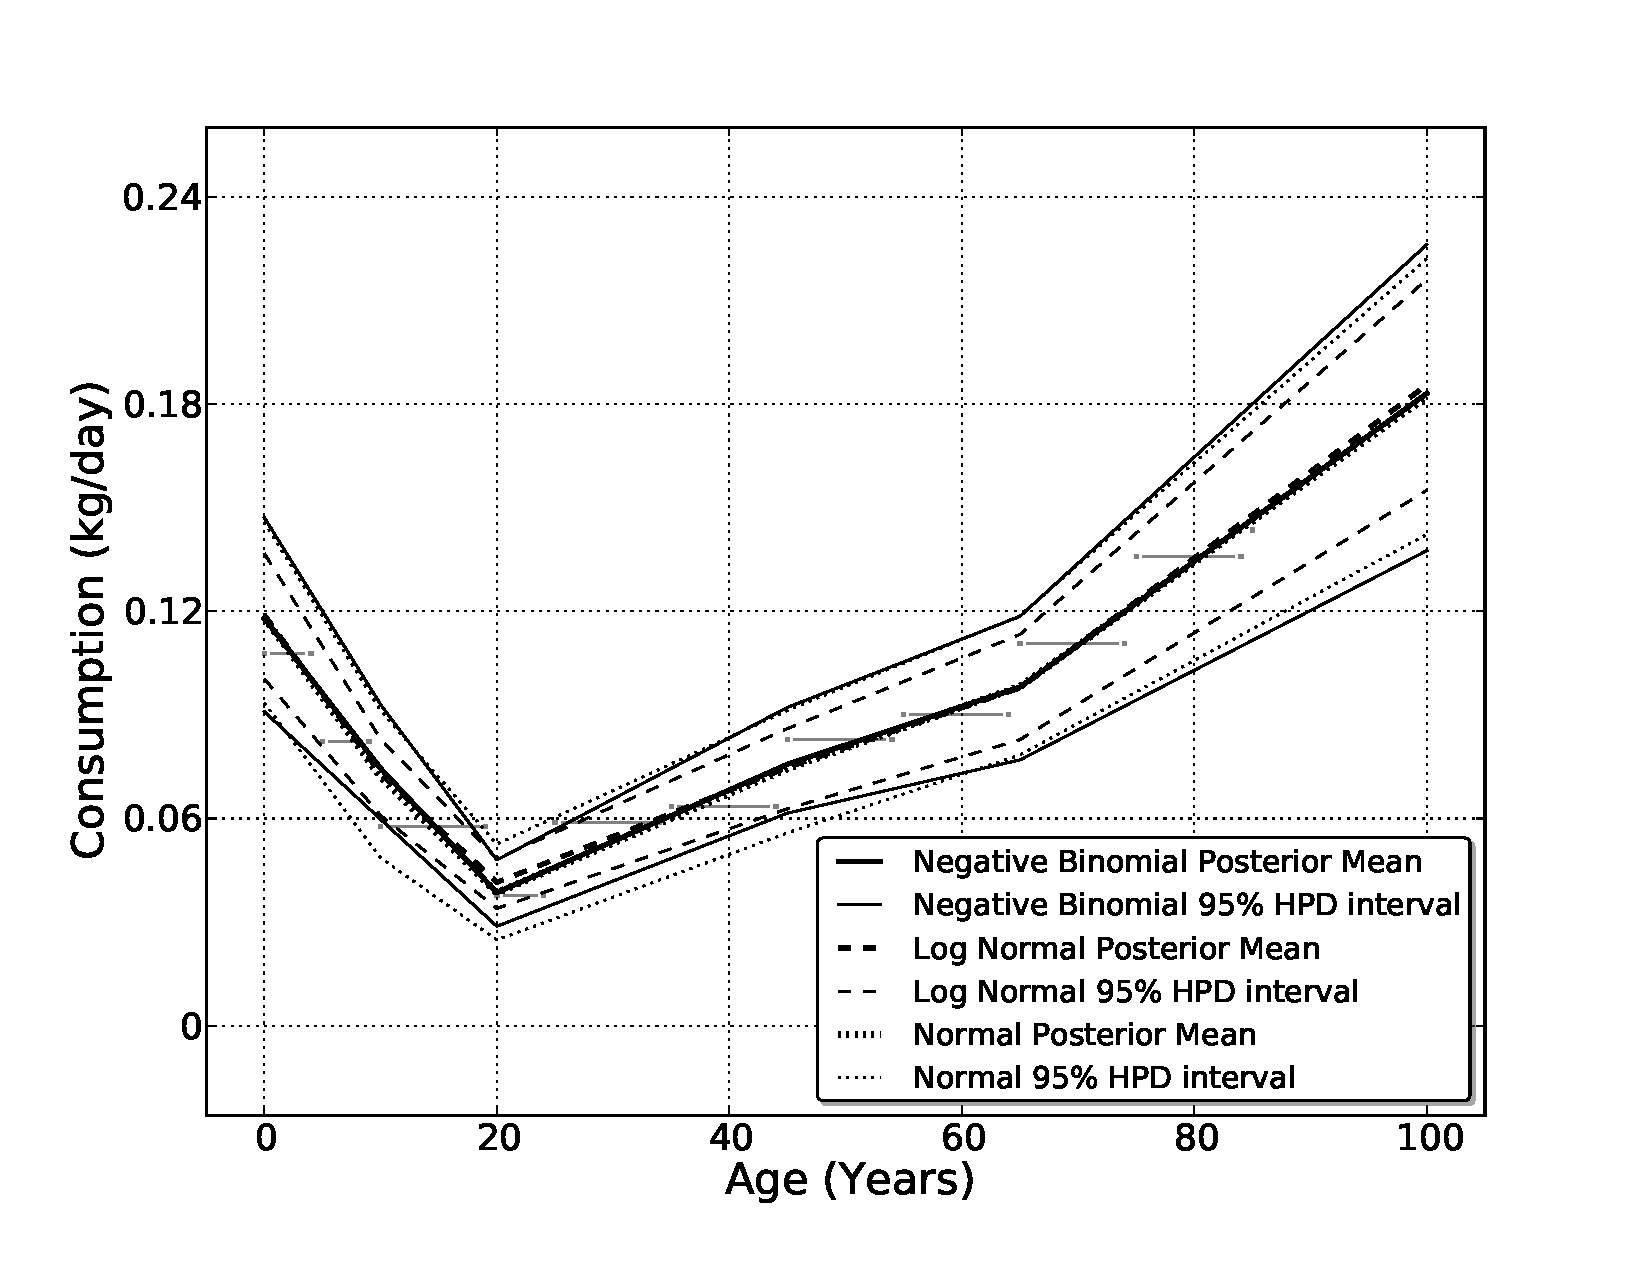
\includegraphics[width=\textwidth]{fruit-rate_type.pdf}
            \caption{Comparison of fruit consumption estimates in
              males in the United States of America in 2005 using the
              negative binomial, log normal and normal rate models.}
            \label{fig:app-fruit rate type}
        \end{center}
    \end{figure}

In a setting where the data is sparser and noisier, the
models still yield quite similar results, as shown in Figure~\ref{fig:app-fruit europe}
for data from Western Europe 2005.  It is worth noting that unlike
the estimates in Figure~\ref{fig:app-fruit europe},
Figure~\ref{fig:app-fruit europe} estimates do not go through the
data at the youngest ages (0-20).  This is because fruit consumption has
substantial country level random effects, shown with a comparison of
Iceland and Greece in Figure~\ref{fig:app-fruit countries}.

    \begin{figure}[h]
        \begin{center}
            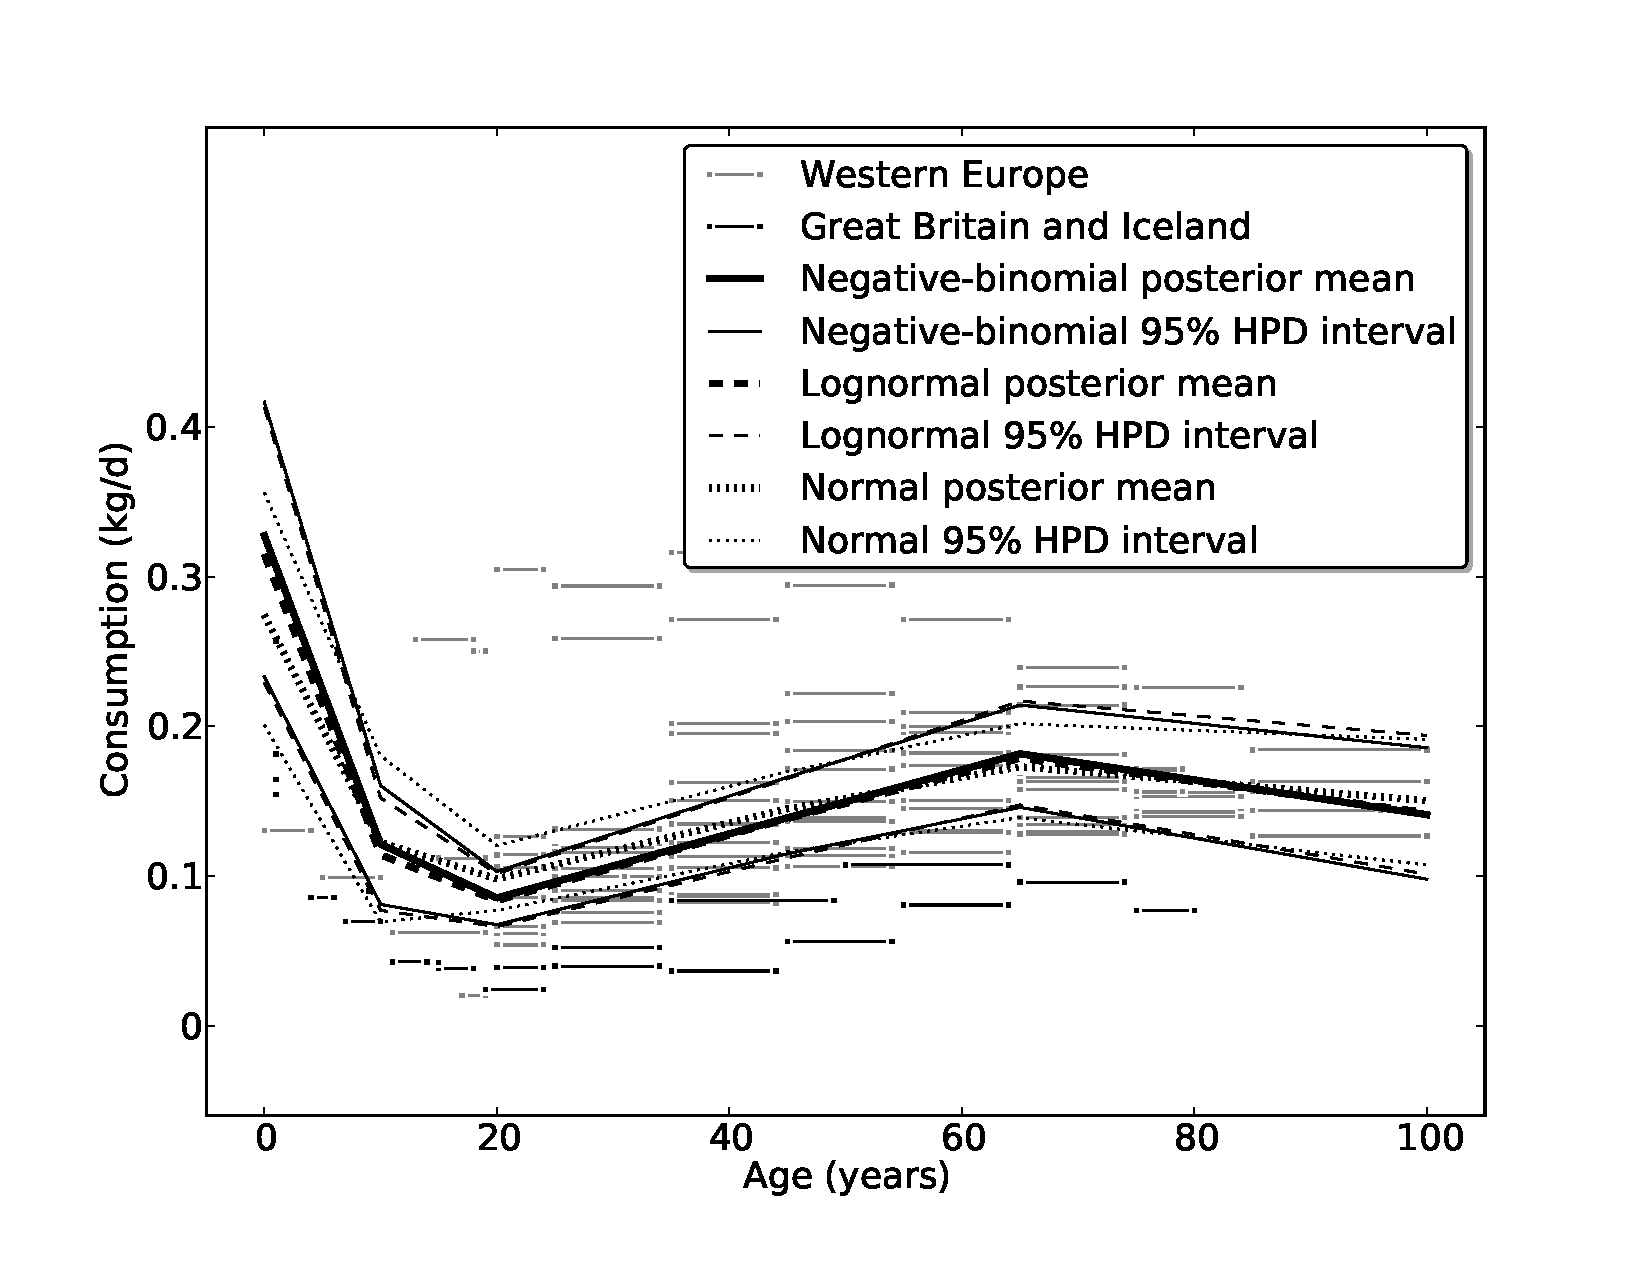
\includegraphics[width=\textwidth]{fruit-we_rate_type.pdf}
            \caption{Comparison of fruit consumption estimates in
              Western European males in 2005 using the
              negative binomial, log normal and normal rate models.}
            \label{fig:app-fruit europe}
        \end{center}
    \end{figure}

    \begin{figure}[h]
        \begin{center}
            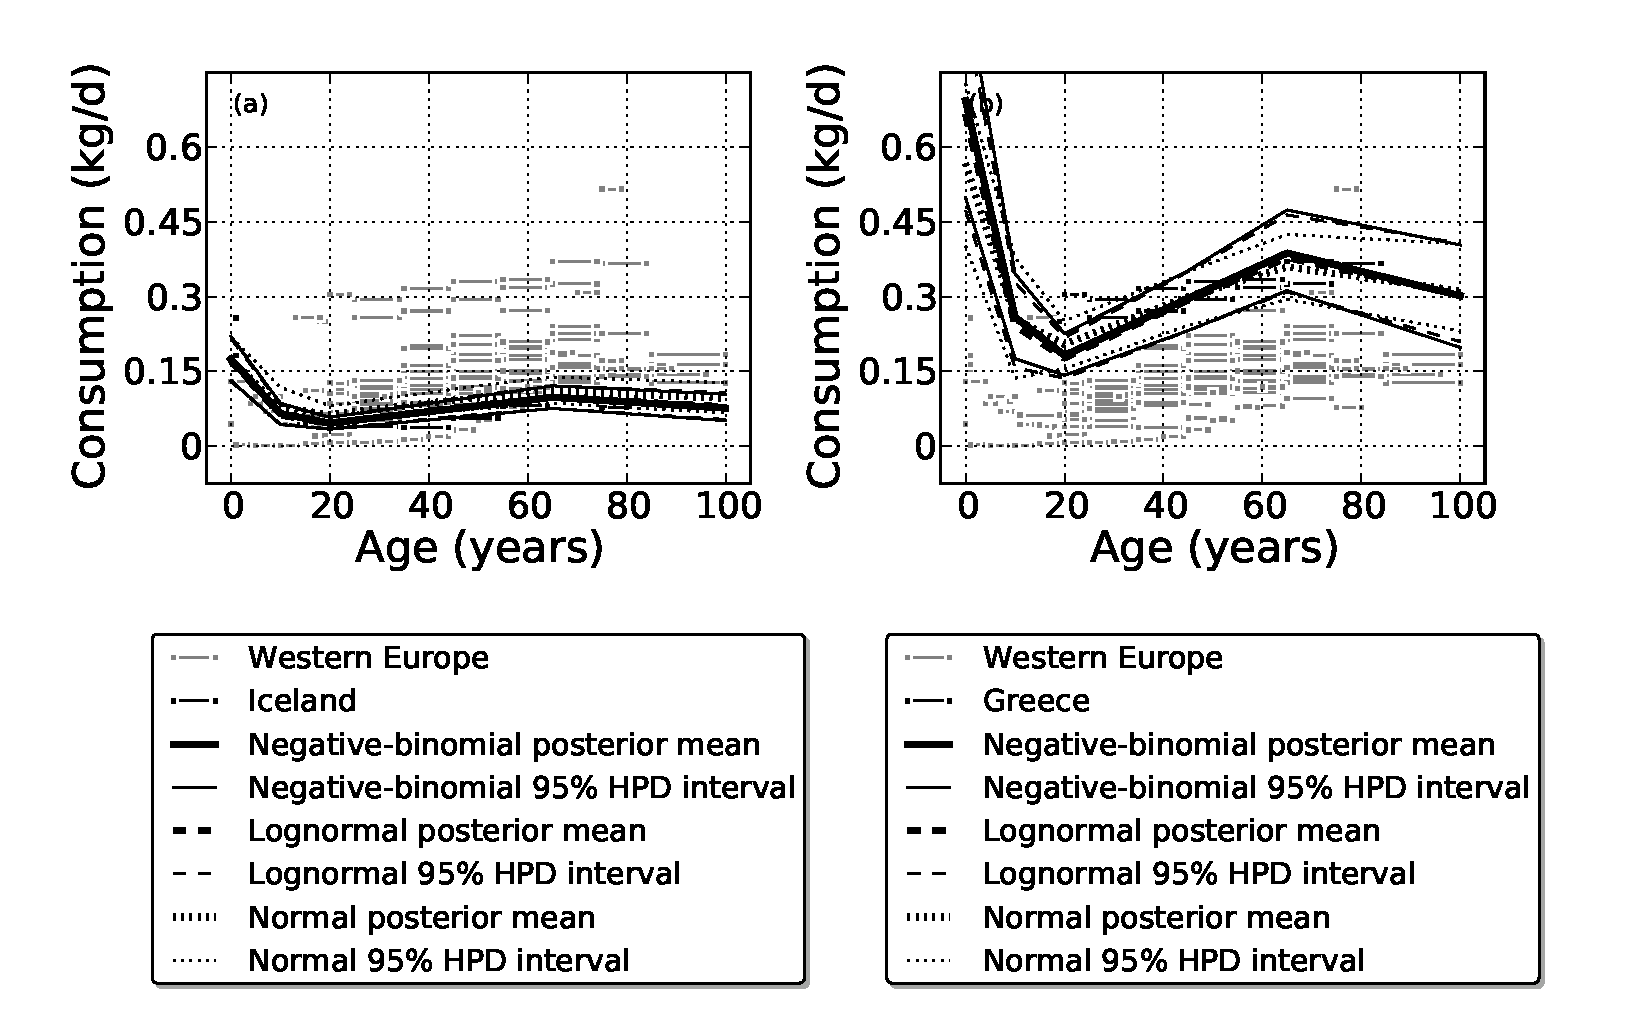
\includegraphics[width=\textwidth]{fruit-isl_rate_type.pdf}
            \caption{Comparison of male fruit consumption estimates in
              (a) Iceland and (b) Greece in 2005 using the
              negative binomial, log normal and normal rate models.}
            \label{fig:app-fruit countries}
        \end{center}
    \end{figure}

From Figure~\ref{fig:app-fruit countries},
small differences in the estimates at the country level are noticeable.
Table~\ref{tab:app-fruit rfx} shows that the mean age-standardized
country estimates differ by rate type.  However, while estimates at
the country level differ slightly, the regional estimate is the same.

    \begin{table}[h]
        \begin{center}
        \begin{tabular}{|c|rl|rl|}
            \hline
                & Iceland&$95\%$ UI & Greece&$95\%$ UI \\
            \hline
                negative binomial & $-0.58$&$ [-0.8, -0.4]$ & $0.80$&$ [0.6, 1.0]$ \\
                normal & $-0.41$&$ [-0.6, -0.2]$ & $0.78$&$ [0.7, 0.9]$ \\
                log normal & $-0.56$& $[-0.7, -0.4]$ & $0.80$&$ [0.6, 0.9]$ \\
            \hline
        \end{tabular}
        \end{center}
        \caption{ Age-standardized fruit consumption estimates
          from a hierarchal random effects spline model with differing
          rate models.}
        \label{tab:app-fruit rfx}
    \end{table}

The country-level estimate for Greece also highlights a challenge of
this approach.  Since there is no data from Greece for the youngest
age groups, the model borrows strength from the other countries in the
region.  But since these countries are lower than average in adult
consumption, while Greece is higher, the model predicts very high
consumption in children.  Assuming the same relationship in
country-to-country variation for children as adults seems reasonable
in theory, and indeed there is not data to contradict this, however
the resulting estimates are substantially above any of the levels
measured in the region.  This is suspicious, and certainly justifies
additional investigation.  It could also call for incorporating
additional priors into the model, based on expert knowledge about the
absolute levels, country-to-country variation, or smoothness or
monotonicity of the age pattern.


With ample data, different rate models produce small differences in
moderately noisy data, mostly at the country level.  Similar estimates
from the negative binomial, normal and log normal rate models only
build confidence that the model is not sensitive to choice of these
rate types.  When the data is sparser or noisier, considering the
difference between estimates produced by different models can be a
useful component of a sensitivity analysis.
